\documentclass[../DCM2_Verslag.tex]{subfiles}
\begin{document}


\section{Resultaten}
\subsection{Baseline}
\begin{tabular}{||l|l||}
   	 Testsoort & Bandbreedte \\ & (Mbits/sec)\\
   	 \hline \hline    
   	 UDP RX & 1.07\\
   	 UDP TX & 56.83 \\
   	 TCP TX & 49.64\\
   	 TCP RX & 46.87\\
   	 \hline
	\end{tabular}
 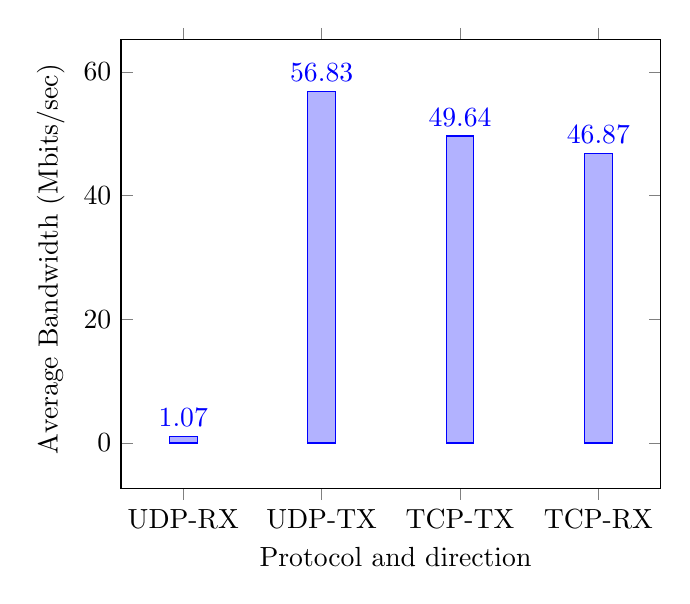
\begin{tikzpicture}[baseline=(current axis.outer east)]
\begin{axis}  
[  
    ybar,  
    enlargelimits=0.15,  
    ylabel={\ Average Bandwidth (Mbits/sec)},  
    xlabel={\ Protocol and direction},  
    symbolic x coords={UDP-RX, UDP-TX, TCP-TX, TCP-RX}, 
    xtick=data,  
    nodes near coords,
    nodes near coords align={vertical},  
]  
\addplot coordinates {(UDP-RX, 1.07) (UDP-TX, 56.83) (TCP-TX,49.64) (TCP-RX,46.87)};  
  
\end{axis}  
\end{tikzpicture}  
\subsection{Window sizes}

\subsubsection{Window sizes test met ESP32 als server}
	\begin{tabular}{||l | l||}
   	 Window size(Kbytes) & Bandbreedte\\ 
   	                     & (Mbits/sec)\\
   	 \hline \hline    
   	 4 KB & 38.53  \\
   	 8 KB & 37.12  \\
   	 16 KB & 35.95 \\
   	 32 KB & 39.54  \\
   	 64 KB & 41.55  \\
   	 128 KB & 42.43  \\
   	 256 KB & 42.84  \\
   	 400 KB & 40.98 \\
   	 \hline
	\end{tabular}
	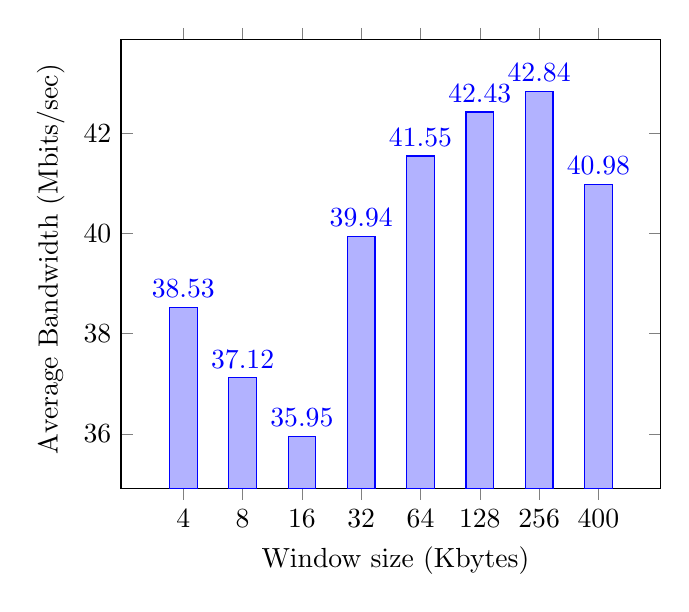
\begin{tikzpicture}[baseline=(current axis.outer east)]
	\begin{axis} [
    ybar= 5pt, 
    symbolic x coords={4,8,16,32,64,128,256,400}, 
    enlargelimits=0.15,   
    ylabel={\ Average Bandwidth (Mbits/sec)},  
    xlabel={\ Window size (Kbytes)},  
    xtick={4,8,16,32,64,128,256,400},  
    nodes near coords,
    nodes near coords align={vertical},  
   ]  
	\addplot coordinates {
    (4,38.53) 
    (8,37.12)
	(16,35.95)
    (32,39.94)
	(64, 41.55)
	(128,42.43)
	(256,42.84)
	(400,40.98)
	};
\end{axis}
\end{tikzpicture}

\subsubsection{Window sizes test met ESP32 als client}
	\begin{tabular}{||l | l||}
   	 Window size(Kbytes) & Bandbreedte\\ 
   	                     & (Mbits/sec)\\
   	 \hline \hline    
   	 4 KB & 4.8  \\
   	 8 KB & 9.32  \\
   	 16 KB & 16.18 \\
   	 32 KB & 26.56  \\
   	 64 KB & 36.76  \\
   	 128 KB & 44.49  \\
   	 256 KB & 43.66  \\
   	 400 KB & 43.9 \\
   	 \hline
	\end{tabular}
	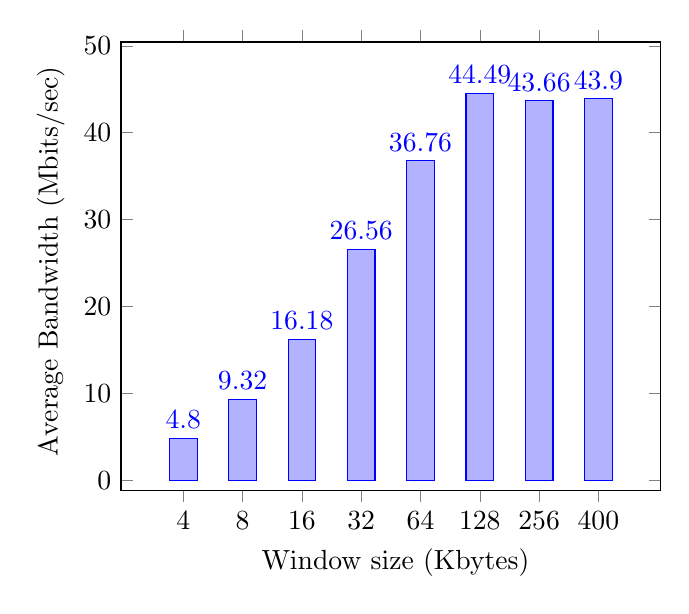
\begin{tikzpicture}[baseline=(current axis.outer east)]
	\begin{axis} [
    ybar= 5pt, 
    symbolic x coords={4,8,16,32,64,128,256,400}, 
    enlargelimits=0.15,   
    ylabel={\ Average Bandwidth (Mbits/sec)},  
    xlabel={\ Window size (Kbytes)},  
    xtick={4,8,16,32,64,128,256,400},  
    nodes near coords,
    nodes near coords align={vertical},  
   ]  
	\addplot coordinates {
    (4,4.8) 
    (8,9.32)
	(16,16.18)
    (32,26.56)
	(64,36.76)
	(128,44.49)
	(256,43.66)
	(400,43.90)
	};
\end{axis}
\end{tikzpicture}

\subsection{Package sizes}


\subsubsection{Package sizes test met ESP32 als server}
	\begin{tabular}{||l | l||}
   	 Package size(bytes) & Bandbreedte\\ 
   	                     & (Mbits/sec)\\
   	 \hline \hline    
   	 200 bytes (160 bytes MSS) &  0.0066\\
   	 400 bytes (360 bytes MSS) &  0.1\\
   	 600 bytes (560 bytes MSS) &  0.35\\
   	 800 bytes (760 bytes MSS) &  32.18\\
   	 1000 bytes (960 bytes MSS) & 34.54\\
   	 1200 bytes (1160 bytes MSS) & 35.64\\
   	 1400 bytes (1360 bytes MSS) & 40.11\\
   	 \hline
	\end{tabular}
	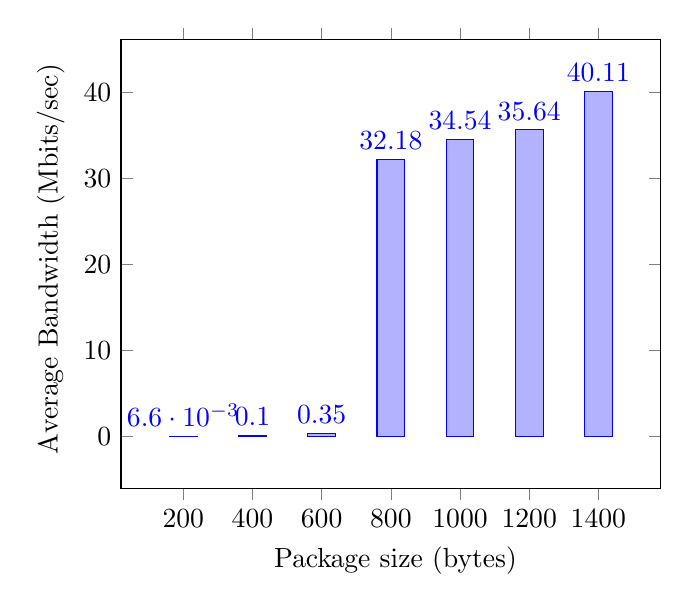
\begin{tikzpicture}[baseline=(current axis.outer east)]
	\begin{axis} [
    ybar= 5pt, 
    symbolic x coords={200,400,600,800,1000,1200,1400}, 
    enlargelimits=0.15,   
    ylabel={\ Average Bandwidth (Mbits/sec)},  
    xlabel={\ Package size (bytes)},  
    xtick={200,400,600,800,1000,1200,1400}, 
    nodes near coords,
    nodes near coords align={vertical},  
   ]  
	\addplot coordinates {
    (200, 0.0066) 
    (400, 0.1)
    (600, 0.35)
	(800, 32.18)
    (1000,34.54)
	(1200,35.64)
	(1400,40.11)
	};
\end{axis}
\end{tikzpicture}

\subsubsection{Package sizes test met ESP32 als client}
	\begin{tabular}{||l | l||}
   	 Package size(bytes) & Bandbreedte\\ 
   	                     & (Mbits/sec)\\
   	 \hline \hline    
   	 200 bytes (160 bytes MSS) &  8.65\\
   	 400 bytes (360 bytes MSS) &  18.58\\
   	 600 bytes (560 bytes MSS) &  35.5\\
   	 800 bytes (760 bytes MSS) &  29.05\\
   	 1000 bytes (960 bytes MSS) & 29.02\\
   	 1200 bytes (1160 bytes MSS) & 24.79\\
   	 1400 bytes (1360 bytes MSS) & 26.97\\
   	 \hline
	\end{tabular}
	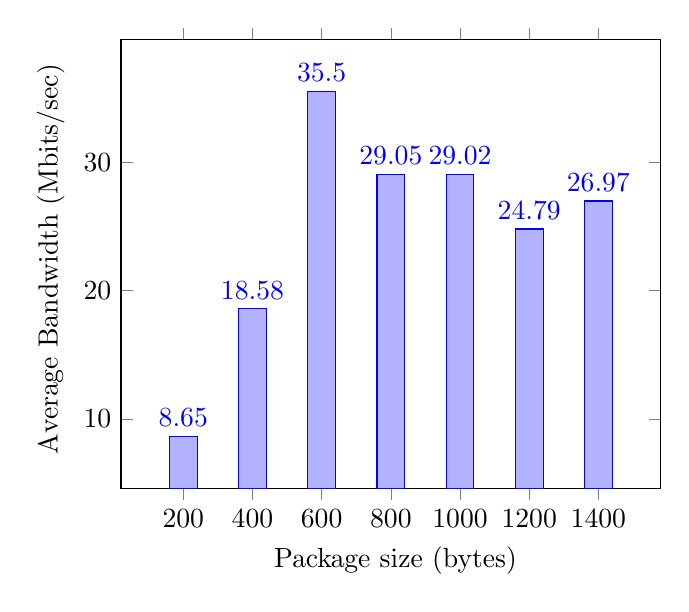
\begin{tikzpicture}[baseline=(current axis.outer east)]
	\begin{axis} [
    ybar= 5pt, 
    symbolic x coords={200,400,600,800,1000,1200,1400}, 
    enlargelimits=0.15,   
    ylabel={\ Average Bandwidth (Mbits/sec)},  
    xlabel={\ Package size (bytes)},  
    xtick={200,400,600,800,1000,1200,1400}, 
    nodes near coords,
    nodes near coords align={vertical},  
   ]  
	\addplot coordinates {
    (200,8.65) 
    (400,18.58)
    (600, 35.5)
	(800, 29.05)
    (1000,29.02)
	(1200, 24.79)
	(1400, 26.97)
	};
\end{axis}
\end{tikzpicture}


\end{document}
